\documentclass[11pt]{article}
% Shared preamble for the pyMack LST documentation set.
% Used by: mean_boundary_layer.tex, disturbance_equations.tex,
%          numerical_methods.tex, validation.tex
% Each document begins with:  \documentclass[11pt]{article}% Shared preamble for the pyMack LST documentation set.
% Used by: mean_boundary_layer.tex, disturbance_equations.tex,
%          numerical_methods.tex, validation.tex
% Each document begins with:  \documentclass[11pt]{article}% Shared preamble for the pyMack LST documentation set.
% Used by: mean_boundary_layer.tex, disturbance_equations.tex,
%          numerical_methods.tex, validation.tex
% Each document begins with:  \documentclass[11pt]{article}\input{lst_preamble}
\usepackage[margin=1in]{geometry}
\usepackage{amsmath,amssymb,mathtools}
\usepackage{booktabs}
\usepackage{enumitem}
\usepackage{array}
\usepackage{graphicx}
\usepackage{caption}
\usepackage{xcolor}
\usepackage[hidelinks]{hyperref}

\graphicspath{{figures/}}
\captionsetup{font=small,labelfont=bf}

\definecolor{kicol}{RGB}{31,143,107}
\definecolor{boxbg}{RGB}{238,246,242}
\definecolor{rmkbg}{RGB}{244,244,244}

\newcommand{\plain}[1]{\par\smallskip\noindent{\color{kicol}\textbf{In plain words.}}\ \textit{#1}\par\smallskip}
\newcommand{\problembox}[1]{%
  \par\smallskip\noindent\fcolorbox{kicol}{boxbg}{%
  \parbox{0.965\linewidth}{\smallskip\textbf{\color{kicol}What problem is solved here.}\ \ #1\smallskip}}\par\smallskip}
\newcommand{\remark}[2]{%
  \par\smallskip\noindent\colorbox{rmkbg}{%
  \parbox{0.965\linewidth}{\smallskip\footnotesize\textbf{#1}\ \ #2\smallskip}}\par\smallskip}
\newcommand{\bridge}[1]{\par\noindent\textit{#1}\par\medskip}

\newcommand{\D}{\mathrm{D}}
\newcommand{\imag}{\mathrm{i}}
\newcommand{\Real}{\operatorname{Re}}
\newcommand{\Imag}{\operatorname{Im}}
\newcommand{\Mae}{M_e}
\newcommand{\Ree}{\mathit{Re}}
\renewcommand{\bar}[1]{\overline{#1}}
\newcommand{\hatu}{\hat{u}}
\newcommand{\hatv}{\hat{v}}
\newcommand{\hatT}{\hat{T}}
\newcommand{\hatp}{\hat{p}}
\newcommand{\hatq}{\hat{q}}
\newcommand{\nuR}{\nu_{\!R}}

\usepackage[margin=1in]{geometry}
\usepackage{amsmath,amssymb,mathtools}
\usepackage{booktabs}
\usepackage{enumitem}
\usepackage{array}
\usepackage{graphicx}
\usepackage{caption}
\usepackage{xcolor}
\usepackage[hidelinks]{hyperref}

\graphicspath{{figures/}}
\captionsetup{font=small,labelfont=bf}

\definecolor{kicol}{RGB}{31,143,107}
\definecolor{boxbg}{RGB}{238,246,242}
\definecolor{rmkbg}{RGB}{244,244,244}

\newcommand{\plain}[1]{\par\smallskip\noindent{\color{kicol}\textbf{In plain words.}}\ \textit{#1}\par\smallskip}
\newcommand{\problembox}[1]{%
  \par\smallskip\noindent\fcolorbox{kicol}{boxbg}{%
  \parbox{0.965\linewidth}{\smallskip\textbf{\color{kicol}What problem is solved here.}\ \ #1\smallskip}}\par\smallskip}
\newcommand{\remark}[2]{%
  \par\smallskip\noindent\colorbox{rmkbg}{%
  \parbox{0.965\linewidth}{\smallskip\footnotesize\textbf{#1}\ \ #2\smallskip}}\par\smallskip}
\newcommand{\bridge}[1]{\par\noindent\textit{#1}\par\medskip}

\newcommand{\D}{\mathrm{D}}
\newcommand{\imag}{\mathrm{i}}
\newcommand{\Real}{\operatorname{Re}}
\newcommand{\Imag}{\operatorname{Im}}
\newcommand{\Mae}{M_e}
\newcommand{\Ree}{\mathit{Re}}
\renewcommand{\bar}[1]{\overline{#1}}
\newcommand{\hatu}{\hat{u}}
\newcommand{\hatv}{\hat{v}}
\newcommand{\hatT}{\hat{T}}
\newcommand{\hatp}{\hat{p}}
\newcommand{\hatq}{\hat{q}}
\newcommand{\nuR}{\nu_{\!R}}

\usepackage[margin=1in]{geometry}
\usepackage{amsmath,amssymb,mathtools}
\usepackage{booktabs}
\usepackage{enumitem}
\usepackage{array}
\usepackage{graphicx}
\usepackage{caption}
\usepackage{xcolor}
\usepackage[hidelinks]{hyperref}

\graphicspath{{figures/}}
\captionsetup{font=small,labelfont=bf}

\definecolor{kicol}{RGB}{31,143,107}
\definecolor{boxbg}{RGB}{238,246,242}
\definecolor{rmkbg}{RGB}{244,244,244}

\newcommand{\plain}[1]{\par\smallskip\noindent{\color{kicol}\textbf{In plain words.}}\ \textit{#1}\par\smallskip}
\newcommand{\problembox}[1]{%
  \par\smallskip\noindent\fcolorbox{kicol}{boxbg}{%
  \parbox{0.965\linewidth}{\smallskip\textbf{\color{kicol}What problem is solved here.}\ \ #1\smallskip}}\par\smallskip}
\newcommand{\remark}[2]{%
  \par\smallskip\noindent\colorbox{rmkbg}{%
  \parbox{0.965\linewidth}{\smallskip\footnotesize\textbf{#1}\ \ #2\smallskip}}\par\smallskip}
\newcommand{\bridge}[1]{\par\noindent\textit{#1}\par\medskip}

\newcommand{\D}{\mathrm{D}}
\newcommand{\imag}{\mathrm{i}}
\newcommand{\Real}{\operatorname{Re}}
\newcommand{\Imag}{\operatorname{Im}}
\newcommand{\Mae}{M_e}
\newcommand{\Ree}{\mathit{Re}}
\renewcommand{\bar}[1]{\overline{#1}}
\newcommand{\hatu}{\hat{u}}
\newcommand{\hatv}{\hat{v}}
\newcommand{\hatT}{\hat{T}}
\newcommand{\hatp}{\hat{p}}
\newcommand{\hatq}{\hat{q}}
\newcommand{\nuR}{\nu_{\!R}}


% \D (from the preamble) is the ordinary wall-normal derivative d/dy used in the
% notation table; \Dmat is the material-derivative operator D/Dt of the governing NS equations.
\providecommand{\Dmat}{\mathrm{D}}

\title{\textbf{The Mean Boundary-Layer Profile}\\[3pt]
\large How \texttt{pyMack} computes the steady laminar compressible base flow\\
whose profiles become the coefficients of the stability equations}
\author{Personal reference note}
\date{\today}

\begin{document}
\maketitle

\begin{abstract}
\noindent Before any stability question can be asked, the disturbance must have something to ride on: a
steady, laminar, compressible boundary layer. This note explains --- assuming no prior exposure --- how
\texttt{pyMack} obtains that base flow. It states the governing compressible Navier--Stokes equations and
their non-dimensionalisation, defines the dimensionless groups and the local Mack length that fix the
solver's units, and then reduces the flat-plate mean flow to a small self-similar boundary-value problem
for the profiles $\bar U(y),\bar T(y),\bar\rho(y),\bar\mu(y)$ and their wall-normal derivatives. Every
equation, boundary condition, coefficient, and default is transcribed from the actual code in
\texttt{pymack/}, cited by file. These profiles --- and, crucially, their $y$-derivatives --- are precisely
the \emph{known coefficients} that enter the linearised disturbance equations, which are derived in the
companion note.
\end{abstract}

\tableofcontents
\bigskip

\noindent\textbf{How to read this.} Boxes marked {\color{kicol}\textbf{``What problem is solved here''}}
state, at each stage, exactly which equation and which boundary conditions are involved. \emph{In plain
words} notes give the intuition; grey \textsf{Remark} asides hold secondary or fallback detail you can skip
on a first read.

\paragraph{Notation.} Overbars are mean (base-flow) quantities. A prime on a mean quantity is
$\D\equiv\mathrm d/\mathrm dy$ (or $\mathrm d/\mathrm d\eta$ in the similarity coordinate, as noted in
context). The rows below cover only the base-flow, transport, and scale symbols this note uses; the
disturbance/eigenvalue symbols live in the companion notes.
\begin{center}\footnotesize
\renewcommand{\arraystretch}{1.18}
\begin{tabular}{@{}ll@{}}
\toprule
\multicolumn{2}{@{}l}{\textbf{Base flow \& transport}}\\
$\bar U,\bar T,\bar\rho{=}1/\bar T$ & mean velocity, temperature, density\\
$\bar\mu,\bar\kappa$ & viscosity, conductivity\\
$C{=}\bar\mu/\bar T,\ K,\ B$ & transport groups, \S\ref{sec:base}\\
\midrule
\multicolumn{2}{@{}l}{\textbf{Scales \& parameters}}\\
$\Mae,\ \Ree,\ \mathit{Pr},\ \gamma$ & Mach, Reynolds, Prandtl, $c_p/c_v$\\
$R_g,\ a_e$ & specific gas constant, edge sound speed ($a_e^2{=}\gamma R_g T_e$)\\
$L^*{=}\sqrt{\nu_e x/U_e}$ & Mack length, Eq.~\eqref{eq:Lstar}\\
$R{=}\sqrt{Re_x},\ F$ & Mack Reynolds, reduced frequency, Eq.~\eqref{eq:RF}\\
$\alpha,\ \alpha_L{=}\alpha L^*,\ \delta^*,\theta$ & streamwise wavenumber, scaled wavenumber, displacement/momentum thickness\\
\bottomrule
\end{tabular}
\end{center}

\bridge{The disturbance rides on a steady laminar flow, so we need that flow --- and its $y$-derivatives ---
before anything else. This note computes it.}

%=====================================================================
\section{Governing equations and non-dimensionalisation}\label{sec:gov}
%=====================================================================
The flow obeys the compressible Navier--Stokes equations --- conservation of mass, momentum, and energy for
a viscous, heat-conducting perfect gas:
\begin{align}
  \frac{\Dmat\rho}{\Dmat t}+\rho\,\nabla\!\cdot\!\mathbf u &= 0, &&\text{(mass)}\label{eq:ns-mass}\\
  \rho\frac{\Dmat\mathbf u}{\Dmat t} &= -\nabla p+\nabla\!\cdot\!\boldsymbol\tau, &&\text{(momentum)}\label{eq:ns-mom}\\
  \rho\,c_p\frac{\Dmat T}{\Dmat t} &= \frac{\Dmat p}{\Dmat t}+\nabla\!\cdot(\kappa\nabla T)+\Phi, &&\text{(energy)}\label{eq:ns-energy}\\
  p &= \rho\,R_g\,T, &&\text{(state)}\label{eq:ns-state}
\end{align}
where $\mathbf u=(u,v)$ is velocity, $\rho$ density, $T$ temperature, $p$ pressure, $\mu$ viscosity,
$\kappa$ conductivity, $c_p$ specific heat, $R_g$ the specific gas constant (plain $R$ is reserved for the
Mack Reynolds number, Eq.~\eqref{eq:RF}), and $\Dmat/\Dmat t=\partial_t+\mathbf u\!\cdot\!\nabla$
the material derivative. The two remaining symbols are the Newtonian \textbf{viscous stress tensor} and the
\textbf{dissipation function},
\begin{equation}\label{eq:tauphi}
  \boldsymbol\tau=\mu\Big(\nabla\mathbf u+\nabla\mathbf u^{\mathsf T}-\tfrac23(\nabla\!\cdot\!\mathbf u)\,\mathbf I\Big),
  \qquad \Phi=\boldsymbol\tau\!:\!\nabla\mathbf u .
\end{equation}
We will not need their closed form again: all that matters downstream is that they are linear in velocity
gradients. These four equations are applied \emph{twice} --- once to obtain the steady mean flow (this
note), once linearised for the disturbance (the companion note).

\begin{figure}[h]\centering
  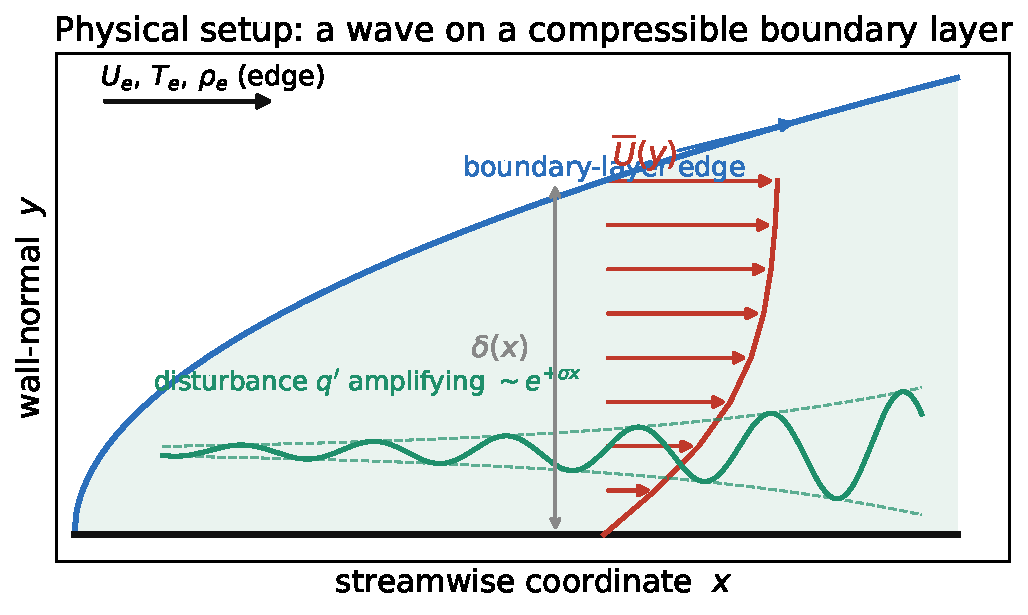
\includegraphics[width=0.86\linewidth]{fig_setup.pdf}
  \caption{The physical setup. A steady compressible boundary layer grows along a wall; its mean velocity
  $\bar U(y)$ and temperature $\bar T(y)$ vary across the layer of thickness $\delta(x)$. Stability theory
  tracks one small disturbance $q'(x,y,t)$ riding in this layer and asks whether it amplifies downstream ---
  but first the mean profiles $\bar U,\bar T$ must be computed, which is the subject of this note.}\label{fig:setup}
\end{figure}

\paragraph{Non-dimensionalisation and default gas constants.} Velocities are scaled by the edge speed
$U_e$, temperature by $T_e$, density by $\rho_e$, viscosity by $\mu_e$, pressure by $\rho_e U_e^2$. Because
the gas is perfect and pressure is nearly uniform across the layer, $\bar\rho=1/\bar T$ in these units.
Three dimensionless groups control everything,
\begin{equation}
  \Mae=\frac{U_e}{a_e},\quad a_e=\sqrt{\gamma R_g T_e},\qquad
  \Ree=\frac{\rho_e U_e L_{\mathrm{ref}}}{\mu_e},\qquad
  \mathit{Pr}=\frac{\mu_e c_p}{\kappa_e},
\end{equation}
where $a_e$ is the edge speed of sound and $R_g$ the specific gas constant, with default air values
$\gamma=1.4$, $\mathit{Pr}=0.72$, Sutherland constant $S=110.4~\mathrm K$, and power-law exponent
$\omega_\mu\approx0.7$ when the power-law viscosity is used.

\paragraph{The Mack length and Reynolds scales.}\label{sec:Lstar} Boundary layers grow like $\sqrt x$, so
the natural local scale at station $x$ is
\begin{equation}\label{eq:Lstar}
  L^*=\sqrt{\frac{\nu_e\,x}{U_e}},\qquad \nu_e=\frac{\mu_e}{\rho_e}.
\end{equation}
With $L_{\mathrm{ref}}=L^*$ the Reynolds number becomes the square root of the usual one, and a fixed
physical frequency $f$ maps to a reduced frequency $F$ (both consumed later, by the neutral-curve and
$N$-factor computations in the companion notes):
\begin{equation}\label{eq:RF}
  R=\frac{U_eL^*}{\nu_e}=\sqrt{Re_x},\quad Re_x=\frac{U_ex}{\nu_e};\qquad
  F=\frac{2\pi f\,\nu_e}{U_e^2};\qquad \alpha_L=\alpha L^* ,
\end{equation}
where $\alpha$ is the streamwise wavenumber. $R$ is the horizontal axis of every neutral curve and
$\alpha_L$ the vertical axis. Conversions live in
\texttt{pymack/scales.py}; the solver itself is dimensionless. A profile may be stored on a $y/\delta^*$ or
a $y/L^*$ grid; the constant $\delta^*/L^*$ converts between them, with $\D\!\mapsto\!(\delta^*/L^*)^{-1}\D$.

%=====================================================================
\section{The base flow}\label{sec:base}
%=====================================================================
\problembox{Solve a \emph{boundary-value problem} (BVP) --- not an eigenvalue problem --- for the steady
laminar profiles $\bar U(y),\bar T(y),\bar\rho(y),\bar\mu(y)$ and their $y$-derivatives. A BVP fixes the
data at both ends ($y=0$ and $y\to\infty$) and has a single solution; an eigenvalue problem instead leaves
a parameter free and asks for the special values that admit a non-zero solution. These profiles become the
known coefficients of the disturbance equations.}

For a flat plate the mean flow is \emph{self-similar}: profiles at different $x$ collapse onto one curve in
a stretched coordinate $\eta$. With the dimensionless stream function $f(\eta)$, $f'=\bar U=u/U_e$ (a prime
is $\mathrm d/\mathrm d\eta$), momentum and energy reduce to two coupled ODEs,
\begin{align}
  \big(C\,f''\big)' + f\,f'' &= 0, \label{eq:bl-mom}\\
  \big(B\,\bar T{}'\big)' + f\,\bar T{}' + (\gamma-1)\,\Mae^2\,C\,\big(f''\big)^2 &= 0, \label{eq:bl-energy}
\end{align}
with transport groups
\begin{equation}\label{eq:transport}
  C=\frac{\mu/\mu_e}{T/T_e}\ \text{(Chapman--Rubesin)},\qquad K=\frac{\kappa}{c_p\mu_e},\qquad
  B=\frac{K}{\bar T}\Big(=\tfrac{C}{\mathit{Pr}}\ \text{at constant }\mathit{Pr}\Big).
\end{equation}
The last term in \eqref{eq:bl-energy} is aerodynamic heating --- it makes a hypersonic layer hot near the
wall and couples energy to velocity. The conductivity model is $\kappa=\mu c_p/\mathit{Pr}$ (so
$\bar\kappa=\bar\mu/\mathit{Pr}$ at constant $\mathit{Pr}$); the transport derivatives
$\mathrm d\mu/\mathrm dT$ etc.\ are taken analytically from the chosen viscosity law.

\paragraph{Wall and edge conditions.}
\begin{equation}\label{eq:blbc}
  \underbrace{f(0)=0,\ f'(0)=0}_{\text{no slip}},\quad
  \underbrace{f'(\infty)=1,\ \bar T(\infty)=1}_{\text{match the edge}},\qquad
  \begin{cases}\bar T{}'(0)=0 &\text{(adiabatic wall)}\\ \bar T(0)=T_w/T_e &\text{(isothermal wall)}\end{cases}
\end{equation}
For an adiabatic wall the recovered temperature is the standard result (stated, not derived)
$T_{aw}/T_e=1+\tfrac12(\gamma-1)\sqrt{\mathit{Pr}}\,\Mae^2$. (For a cone, the edge state itself comes
first, from the Taylor--Maccoll equation behind the conical shock --- a separate calculation, outside
\texttt{pymack/}, in the Sivasubramanian--Fasel cone verification case; not detailed further here. See
\texttt{taylor\_\allowbreak maccoll\_\allowbreak edge\_\allowbreak state.py}.)

\paragraph{Solution and the coordinate transform.} Equations \eqref{eq:bl-mom}--\eqref{eq:bl-energy} are
solved as a 5-state first-order system $[\,f,\bar U,\bar U',\bar T,\bar T'\,]$ by collocation and Newton
iteration (\texttt{scipy.integrate.solve\_bvp}), integrated to $\eta_{\max}\!\approx\!40$ (well beyond the
edge). The implementation is \texttt{pymack/baseflow.py}. The similarity coordinate maps to the physical one
by
\begin{equation}\label{eq:ytransform}
  \frac{y}{L^*}=\sqrt2\!\int_0^\eta\frac{\bar T}{T_e}\,\mathrm d\eta',\quad
  \frac{\delta^*}{L^*}=\sqrt2\!\int_0^\infty(\bar T-\bar U)\,\mathrm d\eta,\quad
  \frac{\theta}{L^*}=\sqrt2\!\int_0^\infty\bar U(1-\bar U)\,\mathrm d\eta,
\end{equation}
where the displacement thickness $\delta^*$ measures how far the wall effectively pushes the outer flow
outward and the momentum thickness $\theta$ the momentum deficit. Figure~\ref{fig:baseflow} (right panel)
plots this transform directly: because $\bar T$ is elevated near the wall, the map from a uniform $\eta$
mesh to physical $y$ is nonlinear, stretching resolution into the hot near-wall region. The solver returns,
on any grid,
$\bar U,\bar U',\bar U'',\ \bar T,\bar T',\bar T'',\ \bar\rho,\ \bar\mu,\ \mathrm d\mu/\mathrm dT,\
\mathrm d^2\mu/\mathrm dT^2,\ \bar\kappa,\ \mathrm d\kappa/\mathrm dT,\ \mathrm d^2\kappa/\mathrm dT^2$.

\remark{Two base-flow implementations.}{\texttt{baseflow.py} contains two equivalent self-similar
formulations sharing the 5-ODE structure above. Equations \eqref{eq:bl-mom}--\eqref{eq:bl-energy} and the
$\sqrt2$ transform \eqref{eq:ytransform} are the \texttt{CompressibleBlasiusProfile} form. The temporal
solver and the worked example (in the companion Numerical Methods note) use \texttt{make\_flatplate\_profile}
(\texttt{FlatPlateProfile}; Ozgen \& Kircali transport laws), an alternative normalisation ($f'=\bar U/\bar T$, $\tfrac12$ factors,
$y/L^*=\eta$, no $\sqrt2$). The two give the same physical profiles; only the similarity bookkeeping
differs.}

\begin{figure}[h]\centering
  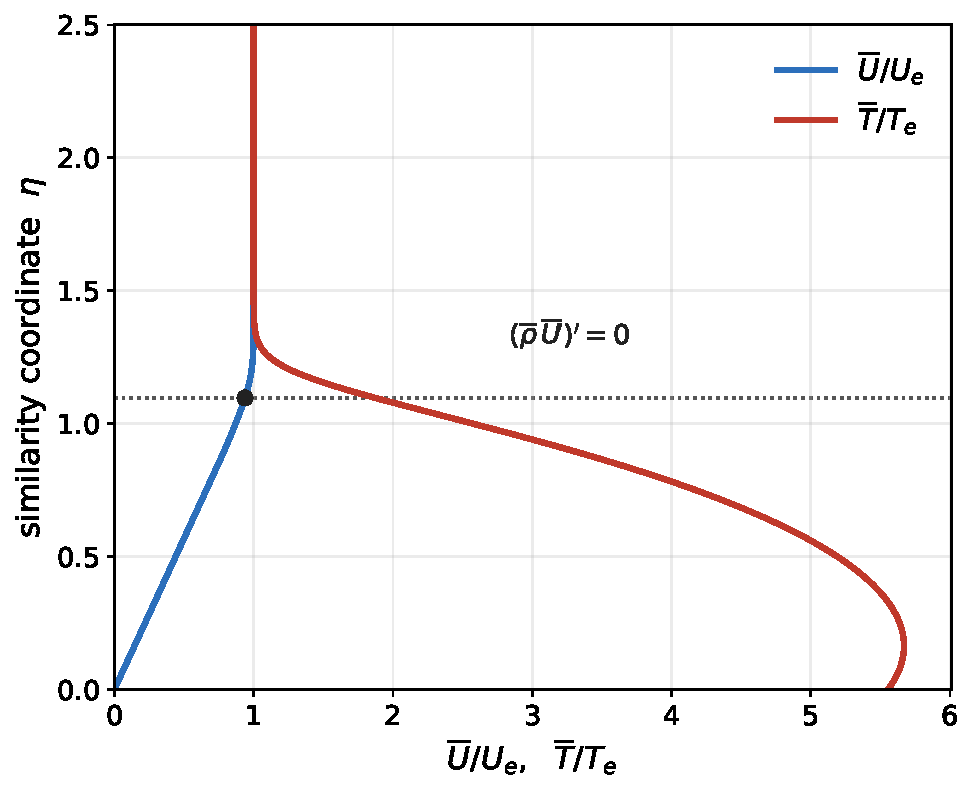
\includegraphics[width=0.86\linewidth]{fig_baseflow.pdf}
  \caption{\emph{Left:} a computed compressible base flow ($\Mae=4.5$, adiabatic). $\bar U(y)/U_e$ rises
  monotonically to the edge; $\bar T(y)$ bulges near the wall from viscous heating. These curves and their
  $y$-derivatives are the known coefficients $\bar U,\bar T,\dots$ in the disturbance equations. The boxed
  callout marks the generalised inflection point, the seat of the inviscid instability (discussed in the
  companion notes on the instability mechanisms). \emph{Right:} the $\eta\to y/L^*$ transform of
  Eq.~\eqref{eq:ytransform}, evaluated for the same case. The solid curve is $y/L^*$ computed by cumulative
  integration of $\bar T$; the dashed grey line is the linear reference $y/L^*=\eta$. Because $\bar T>1$
  near the wall (viscous heating), the transform outpaces the linear reference there: a uniform $\eta$ mesh
  maps to a \emph{stretched} physical mesh close to the wall, which is why $\eta$ rather than $y$ is the
  natural computational coordinate.}\label{fig:baseflow}
\end{figure}

\bridge{These profiles $\bar U(y),\bar T(y),\bar\rho(y),\bar\mu(y)$ and their $y$-derivatives are exactly
the coefficients that appear in the linearised disturbance equations; that linearisation and the resulting
ordinary differential equations are derived in the companion ``Derivation of the Disturbance Equations''
note.}

\end{document}
